% =====================================================================
% Section VII -- The Prefetch Threshold on Its Own
% SpecAsync-UVM manuscript, draft 1 (2026-11-06)
% Every number: paper/support/RESULTS_FACTS.md Section VII (evidence ids
% in the text as \texttt{} for review; strip before submission).
% Stock module 6284DA42 throughout. delta = (t - t51)/t51.
% [WL]   Family B workload names (stencil8k, sweep4k, sweep16k, stream,
%        sgemm, cufft, graphbfs, oversub) -- use the names Section V/the
%        benchmark table defines; "oversub" is the oversubscribed dense
%        stencil cell (XB3). Confirm.
% [FIG]  figure file names from RESULTS_FACTS VII(f); confirm paths.
% =====================================================================

\section{The Prefetch Threshold on Its Own}
\label{sec:threshold}

Section~\ref{sec:spec} found that speculation helps only by making regions pass
the density test sooner. This section measures the test's threshold directly,
on the unmodified driver: first on dense and streaming workloads on two GPUs,
then on a benchmark whose access density we control, then on system-allocated
memory. All comparisons are against the shipped threshold, 51.

\subsection{Dense Access: Faster at a Lower Threshold, on Two GPUs}
\label{sec:thr-dense}

On the RTX~5070~Ti, lowering the threshold to 0 makes Stencil-24K 9.57\% faster,
and to 10, 7.13\% faster (\texttt{E7.A.stencil.*}); the minimum detectable
effects are 1.23\% and 1.28\%. This was the confirmatory test of E7, run after
E6 had found the effect with our module loaded.

Table~\ref{tab:e7} gives the eight further workloads. At threshold 0, four are
significantly faster, by 2.49--16.95\%, and none is significantly slower; the
same holds at 25. The four without a significant change are short runs whose
minimum detectable effects are large, 7--12\% for three of them, so they are
not evidence of no effect; the exception is GraphBFS-23, which runs long,
changes by $-0.26\%$ and could have shown an effect of 0.86\%. The largest gain
is on a dense workload whose array exceeds GPU memory, 16.95\%; a pre-registered
expectation that oversubscription would make the low threshold slower failed
(XB3). For dense access, oversubscription does not reverse the effect.

On the Tesla~T4, with the same driver release, Stencil-24K is 5.07\% faster at
threshold 0 and 3.21\% at 10 (\texttt{T4.A.stencil.*}), and 12 of the 14 further
tests are significantly faster with none slower (\texttt{T4.B.count}). The
oversubscribed workload could not be run there, because the instance's host
memory was smaller than the array (Section~\ref{sec:protocol}). The T4's lower
run-to-run variance makes small effects significant: GraphBFS-23 is 0.14\%
faster, a significant but negligible change.

\begin{table}[t]
\centering
\footnotesize
\caption{Stock driver, threshold 0 against 51 (E7, RTX~5070~Ti).
$\delta$: change in median wall-clock; MDE at the family's level
($m = 16$). Bold: Holm-significant.}
\label{tab:e7}
\input{tables/T-E7}
\end{table}

Tracing shows where the dense gain comes from. On Stencil-24K the bytes moved to
the GPU are the same at both thresholds, within 0.74\%, but the GPU raises
27{,}876 faults at threshold 0 against 91{,}935 at 51 (\texttt{E9.ratio.stencil}).
The lower threshold does not move less data; it moves it in fewer, larger
steps. Part of the gain is not on the GPU at all. The same threshold governs
prefetching when the CPU faults on managed memory (Section~\ref{sec:bg-prefetcher}),
and in every traced run the CPU faults six times less often at threshold 0, all
of them while the host initialises the array (\texttt{E9.ratio.cpu\_faults\_t51\_over\_t0},
\texttt{E9.cpu\_phase.fill\_only}). On the dense cells of our sparse benchmark,
17--23\% of the wall-clock gain falls outside the GPU kernels
(\texttt{E8.outside\_kernels.share\_dense}).

\subsection{Sparse Access: The Lever Cuts Both Ways}
\label{sec:thr-sparse}

The dense results do not say what the low threshold costs when a program uses
only a little of each region. Our sparse benchmark touches $K$ pages per
2\,MB block, chosen at random from a fixed list, over an 8\,GiB array that fits
in GPU memory and a 24\,GiB array that does not. E8 pre-registered a trigger
that would declare the dense-access result not general if any cell with
$K < 512$ was significantly slower at a lower threshold. It fired.

\begin{table}[t]
\centering
\footnotesize
\caption{Sparse benchmark, stock driver, threshold 0 against 51 (E8). $K$:
pages touched per 2\,MB block. Bold: Holm-significant ($m = 16$).}
\label{tab:e8}
\input{tables/T-E8}
\end{table}

With the array in GPU memory the effects are small and mixed: $+3.95\%$ at
$K = 1$ and $-2.32\%$ at $K = 8$, then $-9.69\%$ and $-7.54\%$ at $K = 64$ and
512 (\texttt{E8.in.*}). Once the array exceeds GPU memory, the low threshold is
84.96\% slower at $K = 1$ and 41.15\% slower at $K = 8$, while $K = 64$ and 512
are still 9.67\% and 7.66\% faster (\texttt{E8.ov.*}). At threshold 25 the
$K = 8$ cell is 46.71\% slower and the $K = 1$ cell only 1.88\%. Two
pre-registered expectations about the shape of this pattern failed: the effect
is not monotonic in $K$ (XS4), and threshold 25 does not always lie between 0
and 51 (XS5).

\begin{figure}[t]
\centering
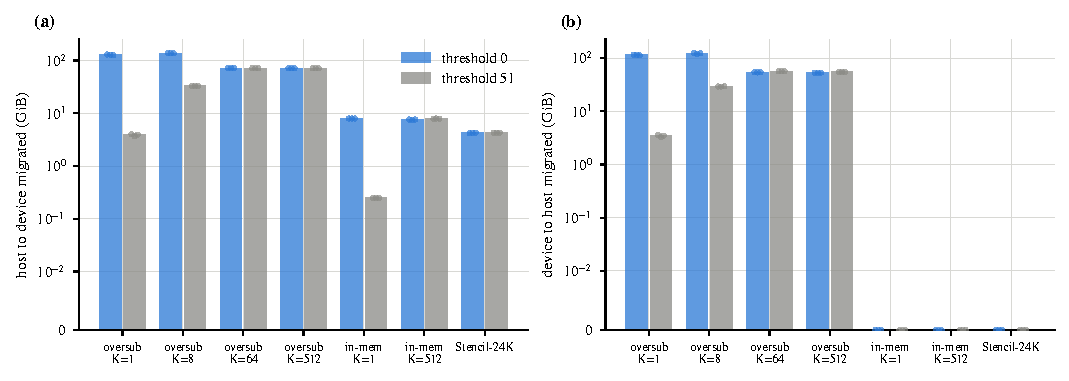
\includegraphics[width=\columnwidth]{figures/fig_e9_migrated_bytes}
\caption{Bytes migrated to and from the GPU per run, by access density and
threshold (E9, nsys, $n = 3$). Oversubscribed, $K = 1$: 129.8\,GiB at
threshold 0 against 3.96\,GiB at 51.}
\label{fig:e9}
\end{figure}

Tracing explains the slowdown (Fig.~\ref{fig:e9}). With the oversubscribed
array and $K = 1$, a run moves 129.8\,GiB to the GPU at threshold 0 and
3.96\,GiB at 51, a factor of 32.8, and almost as much back
(\texttt{E9.cell.ov\_k1.*}). At threshold 0 the first fault in each region
brings in the whole region; with one useful page per block, nearly all of it is
evicted unused and brought back on the next pass. At $K \ge 64$ the traffic is
the same at both thresholds, about 72\,GiB, because the density rule takes whole
regions at 51 too. The slowdown is on the GPU side: the time outside the kernels
falls slightly at threshold 0 even in the slowest cell
(\texttt{E8.outside\_kernels.sparse\_ov}).

\subsection{System-Allocated Memory}
\label{sec:thr-hmm}

On memory allocated with \texttt{malloc}, which the driver services through
HMM (Section~\ref{sec:bg-hmm}), we ran two further gates with arrays that fit in
GPU memory. H1 replicated the dense gain: Stencil-24K is 7.97\% faster at
threshold 0 (\texttt{H1.stencil.*}), less than on managed memory, as it should
be if part of the managed gain was the CPU-side effect above, which HMM does not
share; the two runs are different sessions, so we do not estimate that share
from them.

\begin{figure}[t]
\centering
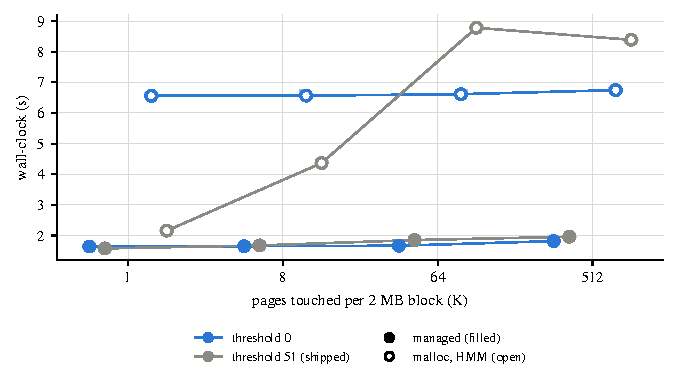
\includegraphics[width=\columnwidth]{figures/F-H2-time}
\caption{Sparse benchmark in GPU memory, by allocator and threshold (H2; 10
runs per cell). Open markers: \texttt{malloc} (HMM); filled: managed.}
\label{fig:h2}
\end{figure}

H1 also found something we had not predicted: with $K = 1$ the low threshold was
about three times slower on HMM, with no oversubscription. H2 pre-registered a
test of an explanation, stating that the hypothesis came after the observation
(Section~\ref{sec:protocol}). Fig.~\ref{fig:h2} shows the result. On HMM, the
time at threshold 0 is the same at every $K$, within 2.8\% (\texttt{H2.Z1}),
because the first fault in each region migrates all of it; at 51 it rises with
$K$. The low threshold is 203.65\% slower at $K = 1$ and 50.39\% slower at $K = 8$,
and 24.66\% and 19.56\% faster at $K = 64$ and 512 (\texttt{H2.malloc\_*}). On
managed memory, in the same session, the same cells change by $+3.92\%$,
$-1.49\%$, $-9.99\%$ and $-7.19\%$ (\texttt{H2.managed\_*}), within a point of
E8's values from an earlier session.

The volume moved does not explain the difference between the allocators. At
threshold 0 a $K = 1$ pass moves essentially the whole array on both: on HMM,
measured as GPU memory in use, 1.03 of the array (\texttt{H2.res.malloc.k1.t0});
on managed memory, measured as traced bytes in E9, 1.00 (\texttt{E9.htod\_frac.in\_k1.t0}).
At 51 the same pass moves 0.061 and 0.031 of it. The cost of moving it differs:
the $K = 1$ slowdown is 199.7 percentage points larger on HMM, with a 95\%
bootstrap interval of 198.1 to 201.7 (\texttt{H2.Z7}). This is consistent with
HMM's migration in 4\,KB units through \texttt{migrate\_vma}, against 2\,MB
chunks for managed memory (Section~\ref{sec:bg-hmm}); H2 does not isolate that
cause. One caution about the measure: on managed memory, GPU memory in use
records allocation, not migration, so we use it for HMM only (catalog
entry~31).

Two limits apply. These are in-memory results; the first oversubscribed HMM
cell crashed the stock driver, and that case was not measured
(Section~\ref{sec:protocol}). And two of H2's expectations about the shape of
the curve at threshold 51 failed (Z2, Z3): at 51, $K = 512$ is faster than
$K = 64$.

\subsection{Summary}

No fixed threshold dominates the shipped one. A low threshold helps dense and
streaming access, on two GPU generations, by moving the same data in fewer
steps and by reducing CPU faults during initialisation. It hurts sparse access
by moving data the program never uses, which costs heavily once the array
exceeds GPU memory and, on system-allocated memory, even before. This is the
trade-off Go \emph{et al.}\ reported \cite{go2023earlyadaptor}; our measurements
replicate it on newer hardware and add the access-density, traced-byte and HMM
dimensions. Section~\ref{sec:discussion} discusses what it implies for a
threshold that adapts.
